\documentclass{scrreprt}
\usepackage[utf8]{inputenc}
\usepackage[T1]{fontenc}
\usepackage[french]{babel}
\KOMAoptions{fontsize=14pt}
\usepackage{graphicx}
\usepackage[a4paper, total={7.5in, 10in}]{geometry}
\usepackage{url}

\title{\textbf{Projet de Modélisation}}
\subtitle{Problèmes de cheminement dans les graphes}
\date{Mars 2018}
\author{Roméo Florian \and Webert Chris}
\begin{document}
	{\small\maketitle}
	\tableofcontents
	\chapter{Problème}
	\section{Données}
	On dispose d'un graphe orienté donné par l'utilisateur. Il peut le créer manuellement via l'interface en ligne de commande, ou bien donner un fichier \textit{GPR}.
	
	Chaque sommet est identifié par une chaîne de caractère unique et contient les bornes inférieures et supérieures de la fenêtre.
	
	Chaque arête est également identifiée par une chaîne de caractère unique et contient deux valuations strictement positives. 
	On considère que la première représente un coût et la seconde la durée.
	
	\section{Traitements}
	Le programme doit être capable de donner plusieurs informations sur le graphe:
	\begin{itemize}
		\item détecter l'existence d'un chemin quelconque entre deux sommets donnés;
		\item détecter l'existence de circuits dans le graphe;
		\item donner les composantes fortement connexes;
		\item donner les numérotations préfixes, suffixes et l'ordre topologique de chaque sommet;
		\item donner le meilleur chemin en fonction:
		\begin{itemize}
			\item du meilleur coût;
			\item de la meilleure durée;
			\item du meilleur coût avec une durée limitée;
			\item de la meilleure durée avec un coût limité
		\end{itemize}
	\end{itemize}

	La plupart des traitements ci-dessus doivent être visualisés graphiquement pour le confort de l'utilisateur.
	
	\chapter{Programmation}
	\section{Algorithmes de traitement}
	Tous les algorithmes de traitement ont été implémentés de manière itérative, permettant de traiter des graphes beaucoup plus volumineux.
	
	\subsection{Parcours de graphe}
	Le parcours en profondeur \textit{DFS (Depth First Search)} a été choisi ici. Il est utilisé pour la numérotation des sommets, l'existence de chemins entre deux sommets, la détection de circuits et des composantes fortement connexes.
	
	\subsection{Recherche de meilleur chemins}
	La recherche du meilleur chemin avec seulement le meilleur coût ou seulement le meilleur temps se fait à l'aide de l'algorithme de Dijkstra. 
	Il a été choisi car les valuations des arcs sont strictement positives.
	
	Cette recherche demande en paramètre une fonction externe qui renvoie la valuation à utiliser. 
	Cela permet de ne pas avoir à dupliquer du code pour chaque nouvelle valuation ajoutée à un arc.
	
	La recherche du meilleur chemin en tenant compte des fenêtres de temps utilise l'algorithme à correction d'étiquettes.
	Nous avons choisi cet algorithme car les corrigés des séances de TD nous ont permit de vérifier son bon fonctionnement.
	
	\subsection{Structure}
	Le diagramme de classe est visible sur la figure~\ref{uml_algo} page~\pageref{uml_algo}.
	La classe \textit{Search} est la base de tout parcours itératif. Elle contient une file des prochains sommets à explorer et appelle les classes filles pour chaque sommet a explorer.
	
	La classe \textit{DisconnectedGraphSearch} permet de parcourir des graphes non connexes. Si demandé, elle vérifiera à la fin du parcours si tous les sommets ont été fermés. Si ce n'est pas le cas, un nouveau parcours sera lancé sur le premier sommet non fermé trouvé.
	
	Les classes \textit{DFS}, \textit{PCC}, \textit{PCCFT} implémentent respectivement les algorithmes de parcours en profondeur, de Dijkstra, et à correction d'étiquette.
	\begin{figure}[!h]
		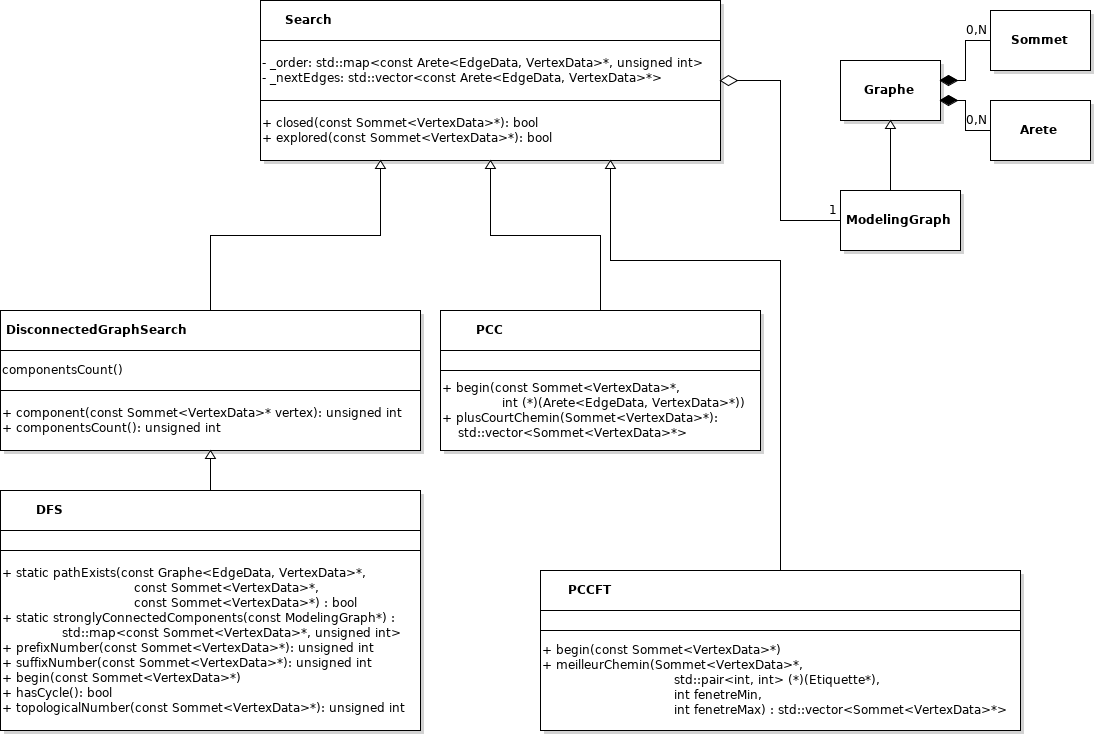
\includegraphics[scale=0.5]{uml_algo}
		\caption{\label{uml_algo} Diagramme de classes des algorithmes}
	\end{figure}
	\newpage

	\section{Lecture de fichiers GPR}
	Le diagramme de classe est visible sur la figure~\ref{uml_gpr} page~\pageref{uml_gpr}.
	Les fichiers \textit{GPR} sont lus par la classe \textit{GPRParser}, associée à une chaîne de responsabilité. Chaque ligne sera lue par \textit{GPRParser}, puis envoyée à la chaîne de responsabilité qui la traitera, si possible.
	
	\begin{figure}[!h]
		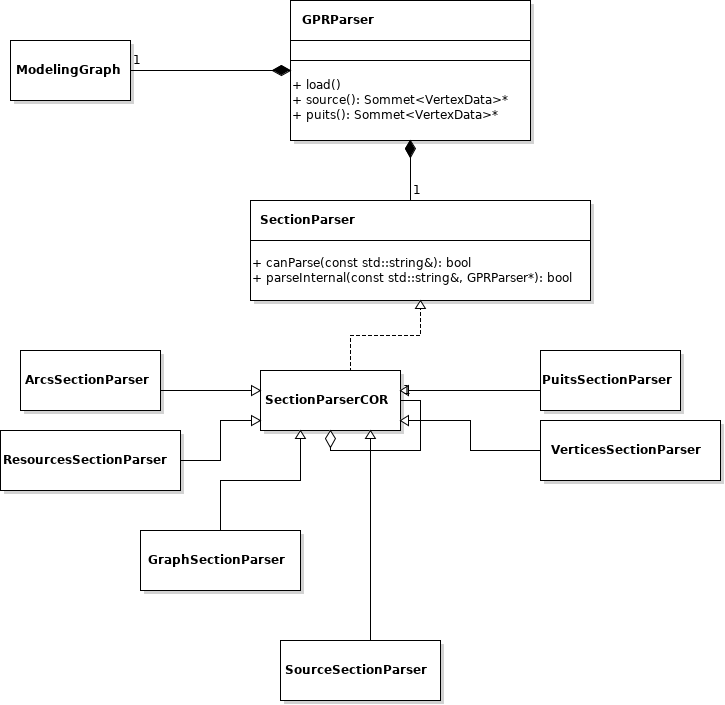
\includegraphics[scale=0.7]{uml_gpr}
		\caption{\label{uml_gpr} Diagramme de classes du lecteur \textit{GPR}}
	\end{figure}
	
	\newpage
	\section{Interface utilisateur}
	L'interface utilisateur a été conçue de façon à ne pas avoir de dépendances sur le projet. Elle utilise la console pour interagir avec l'utilisateur, et crée des fichiers au format \textit{DOT}\footnote{\url{http://www.graphviz.org/pdf/dotguide.pdf}}.
	

	\chapter{Résultats et performances obtenus}
	\section{Performances}
	\begin{center}
		\begin{tabular}{|l|r|r|r|r|r|}
			\hline
			Instance \textit{(nb sommets/nb arcs)} & 10/36 & 20/122 & 50/1086 & 100/1694 & 160/2815 \\
			\hline
			Ouverture ($\mu s$) & 430 & 1011 & 5576 & 8860 & 13114 \\
			\hline
			Visualisation ($\mu s$) & 524 & 990 & 6737 & 8815 & 13235 \\
			\hline
			Parcours DFS ($\mu s$) & 319 & 493 & 2469 & 3460 & 9261 \\
			\hline
			Detection CFC ($\mu s$) & 447 & 1205 & 7052 & 13196 & 23009 \\
			\hline
			PCC ($\mu s$) & 113 & 429 & 11503 & 18236 & 157206 \\
			\hline
			PPC-FT ($\mu s$) & 122 & 1068 & 27489 & 21389 & 42926 \\
			\hline
		\end{tabular}
		\captionof{table}{Résultats des instances \textit{GPR} fournies}
	\end{center}

	Tous les parcours DFS partent de la source, et les recherches du meilleur chemin se font de la source au puits.
	
	\section{Résultats graphiques}
	\subsection{DFS}
	Le rendu est visible sur la figure~\ref{render_dfs} page~\pageref{render_dfs}.
	
	Chaque nœud contient :
	\begin{itemize}
		\item son identifiant;
		\item P: son numéro préfixe;
		\item S: son numéro suffixe
	\end{itemize}

	Les arcs parcourus sont pleinement affichés avec leur ordre de parcours.

	Les nœuds $T_1$…$T_n$ correspondent à l'ordre topologique et sont alignés horizontalement avec le nœud du graphe correspondant.

	\begin{figure}[!h]
		\begin{center}
			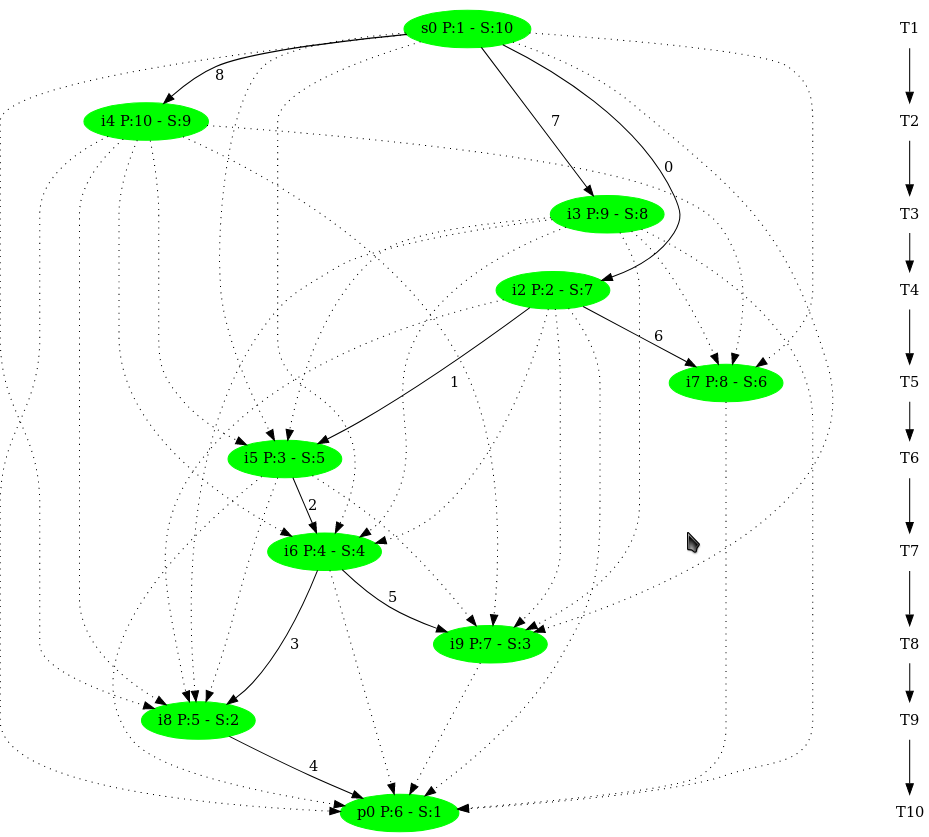
\includegraphics[scale=0.7]{render_dfs}
		\end{center}
		\caption{\label{render_dfs} Rendu du parcours \textit{DFS} de \url{data_VRPTW_10.gpr}}
	\end{figure}

	\newpage
	
	\subsection{Composantes fortement connexes}
	Le rendu est visible sur la figure~\ref{render_scc} page~\pageref{render_scc}.
	
	Chaque nœud contient son identifiant, et est inclus dans le cadre correspondant à une composante fortement connexe.
	
	Les arcs sont affichés pleinement s'ils font partie de la même composante connexe, en pointillés sinon.
	
	\begin{figure}[h]
		\begin{center}
			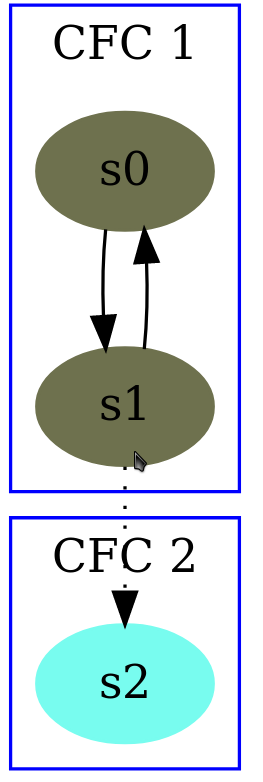
\includegraphics[scale=0.7]{render_scc}
		\end{center}
		\caption{\label{render_scc} Rendu de la recherche de composantes fortement connexes dans \url{data_scc.gpr}}
	\end{figure}
	\newpage
	
	\subsection{Plus court chemin}
	Le rendu est visible sur la figure~\ref{render_pcc} page~\pageref{render_pcc}.
	
	Chaque nœud contient son identifiant, et est affiché en vert s'il fait partie du plus court chemin. Les arcs en faisant partie sont pleinement affichés.
	
	\begin{figure}[h]
		\begin{center}
			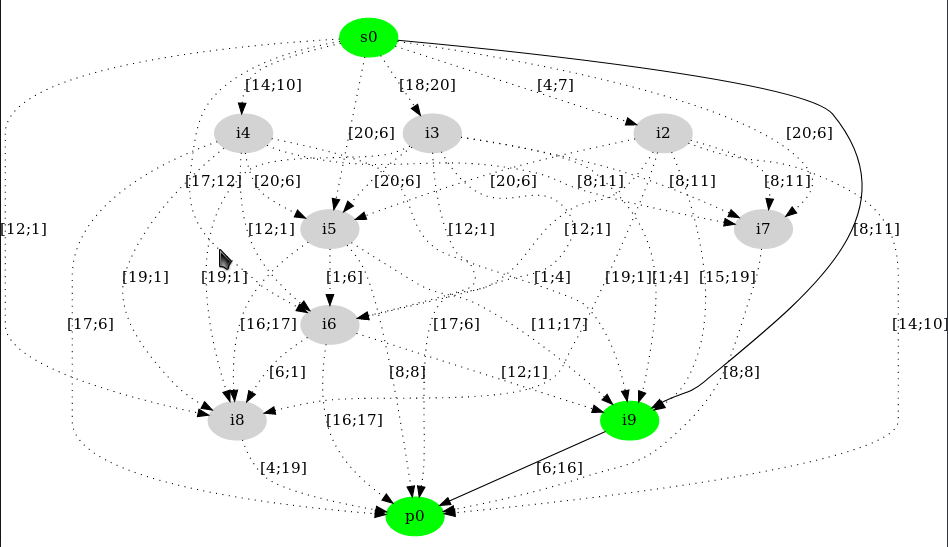
\includegraphics[scale=0.7]{render_pcc}
		\end{center}
		\caption{\label{render_pcc} Rendu de la recherche du plus court chemin de \url{data_VRPTW_10.gpr}}
	\end{figure}
	\newpage
	
\end{document}